%-----------------------------------------
\begin{frame}
\frametitle{Observable for forecast operations}
Still water level.\\
Wave runup, inundation, video: important but not operational yet
\begin{minipage}{0.6\textwidth}
    \begin{figure}      
    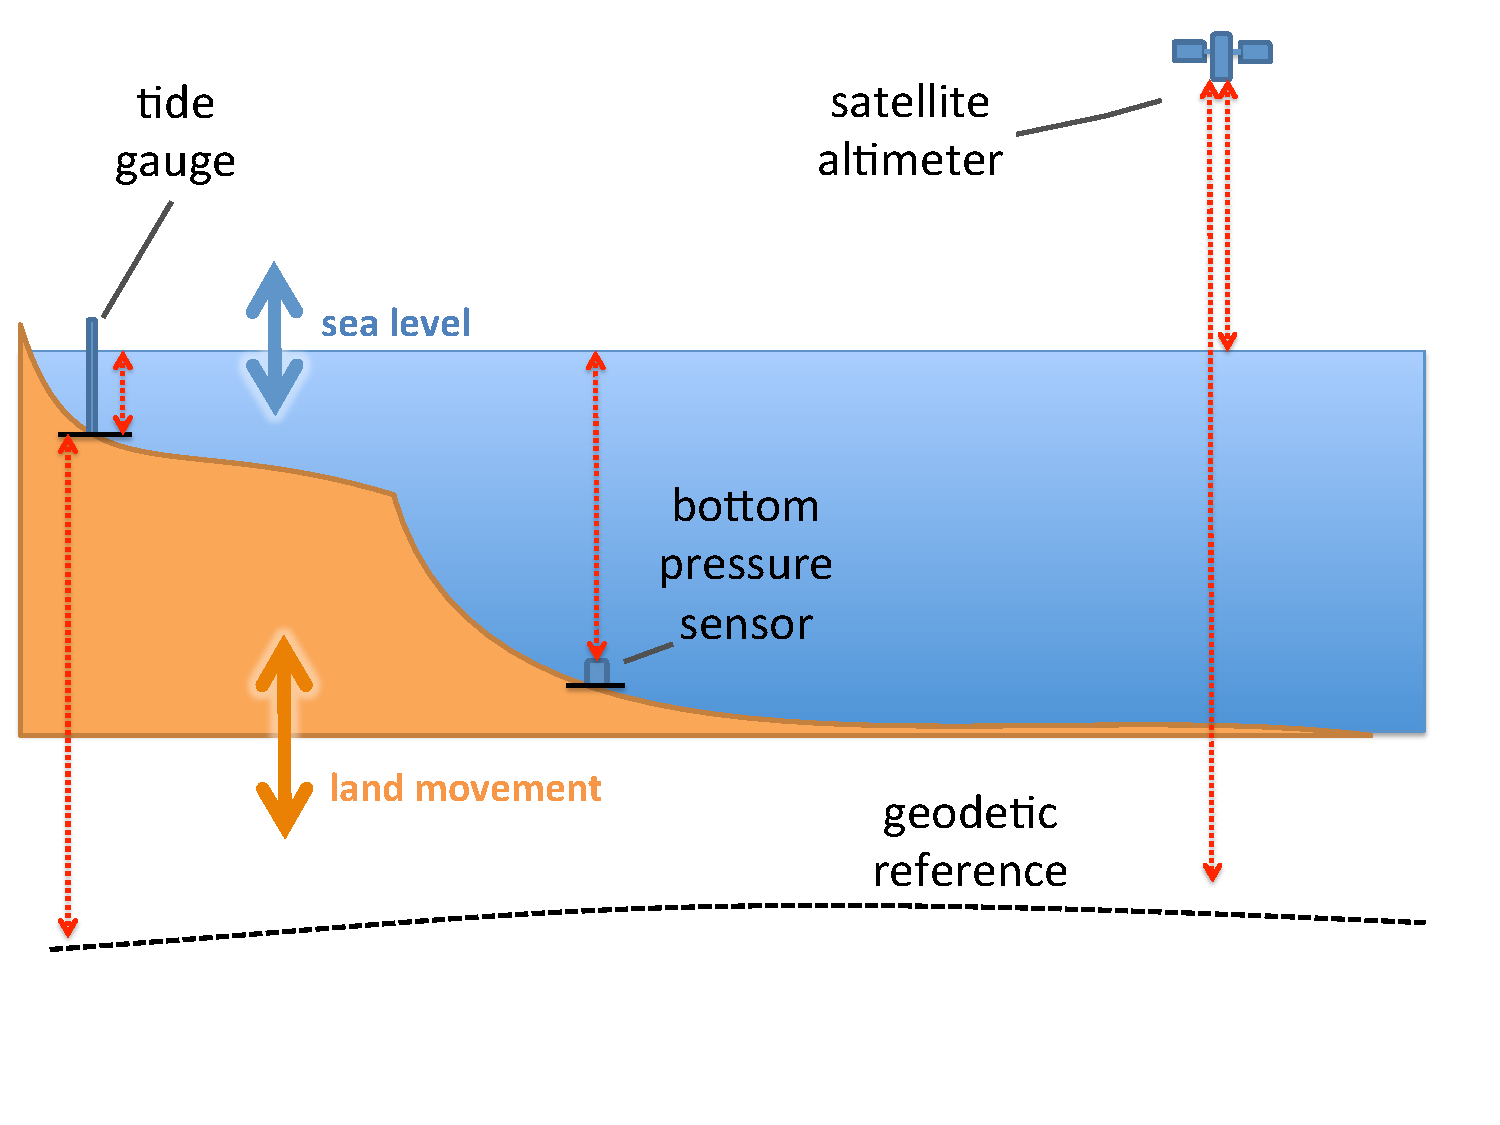
\includegraphics[width=\textwidth]{figures/diagrams/sealevel_cartoon.pdf}
    \end{figure}
\end{minipage}
\begin{minipage}{0.35\textwidth}
    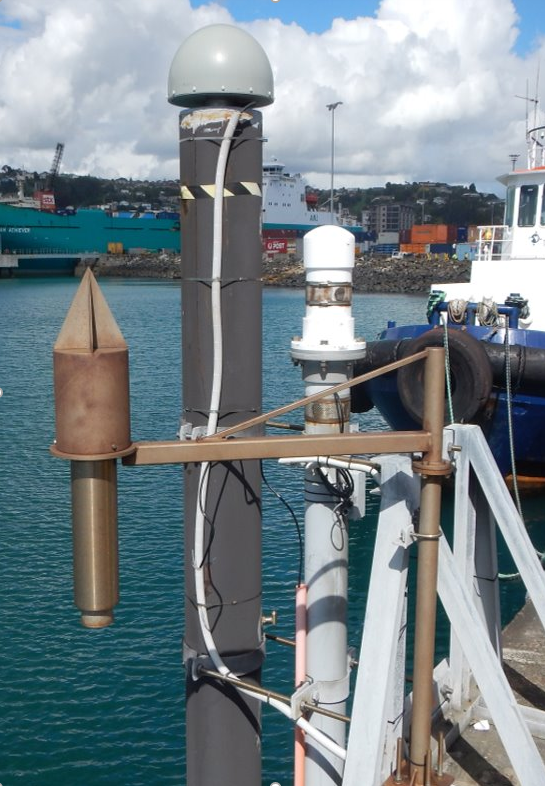
\includegraphics[height=3cm]{figures/images/tidegaugeEg.png}
    \vspace{1cm}
    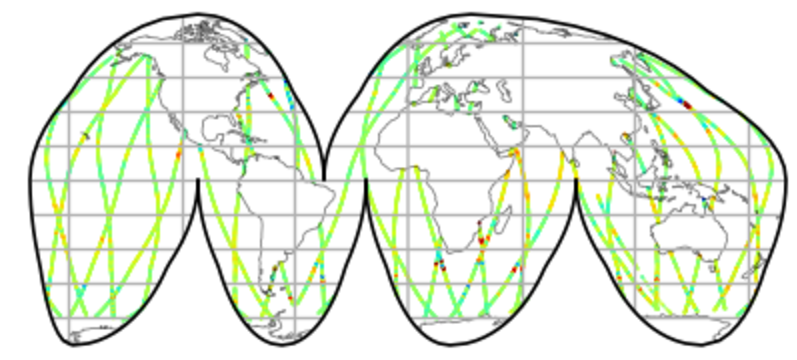
\includegraphics[width=\textwidth]{figures/maps/altimeterCoverageEg.png}
\end{minipage}

\end{frame}
%-----------------------------------------
\begin{frame}
\frametitle{Still water level spectra}
Patterson River Vic
\begin{minipage}{1.0\textwidth}
    \begin{figure}      
    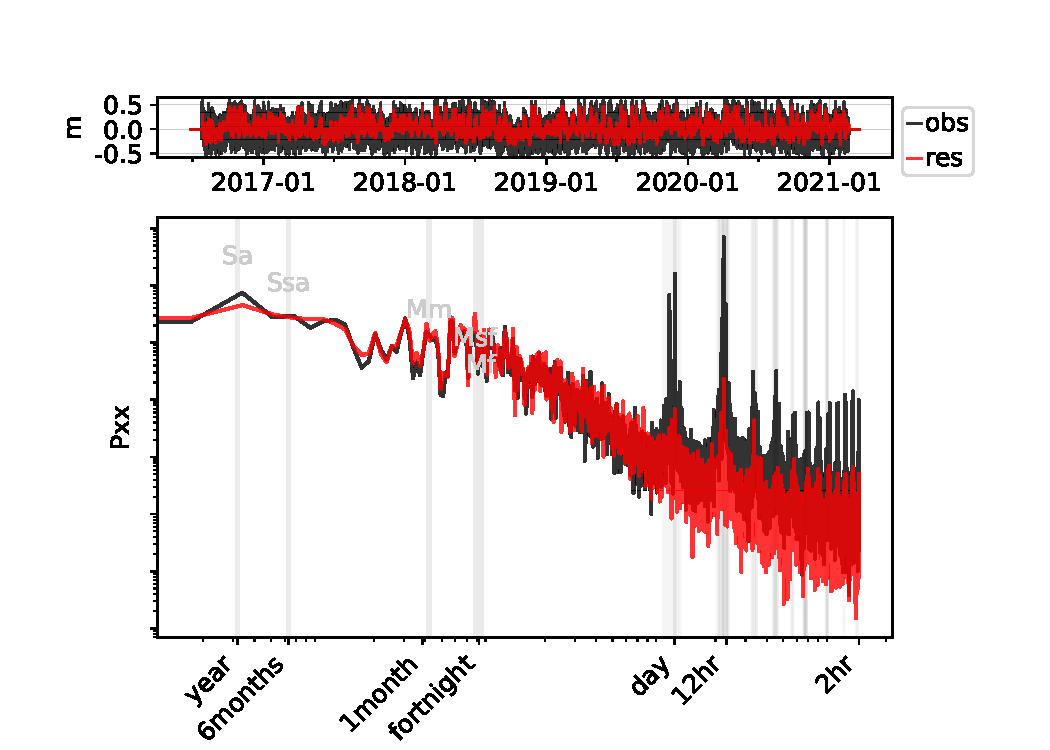
\includegraphics[height=0.8\textheight]{figures/plots/586204_verify_Pxx.pdf}
    \end{figure}
\end{minipage}
\end{frame}
%-----------------------------------------
\begin{frame}
\frametitle{Phenomena scales}
Broadband, mix varies with location.
    \begin{figure}      
    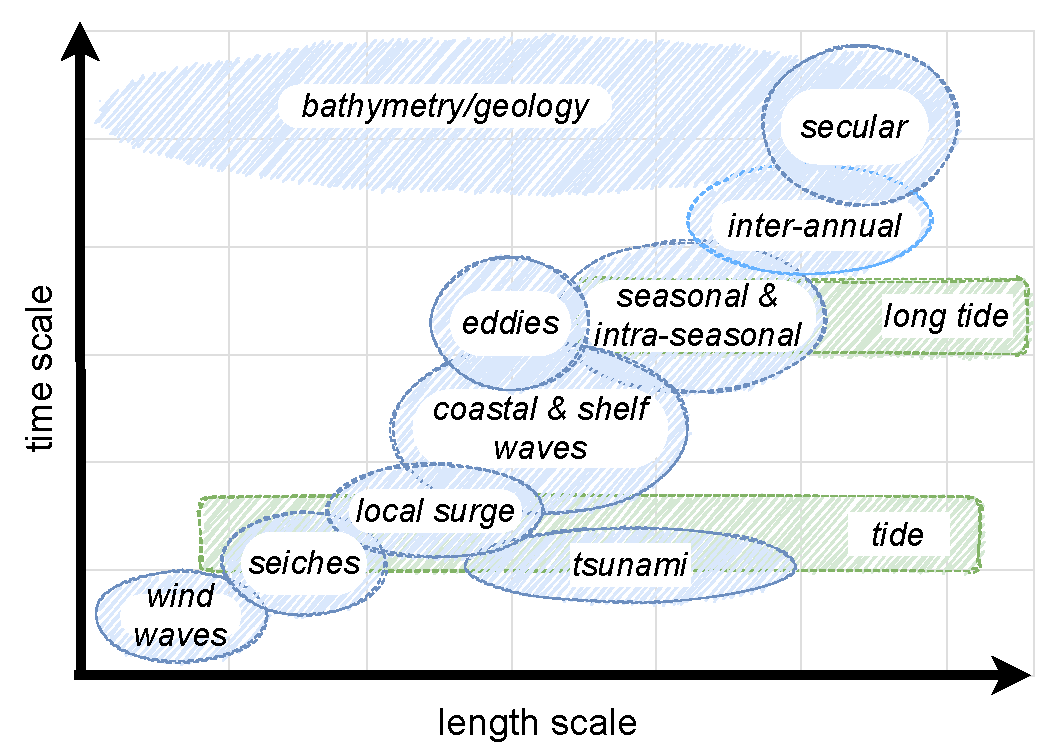
\includegraphics[height=0.8\textheight]{figures/diagrams/scales_time_length.pdf}
    \end{figure}
\end{frame}
%-----------------------------------------
\begin{frame}
\frametitle{Foundational forecast systems}
    Images of models here\\
    Maybe even ROAM diagram.
    %\begin{figure}      
    % 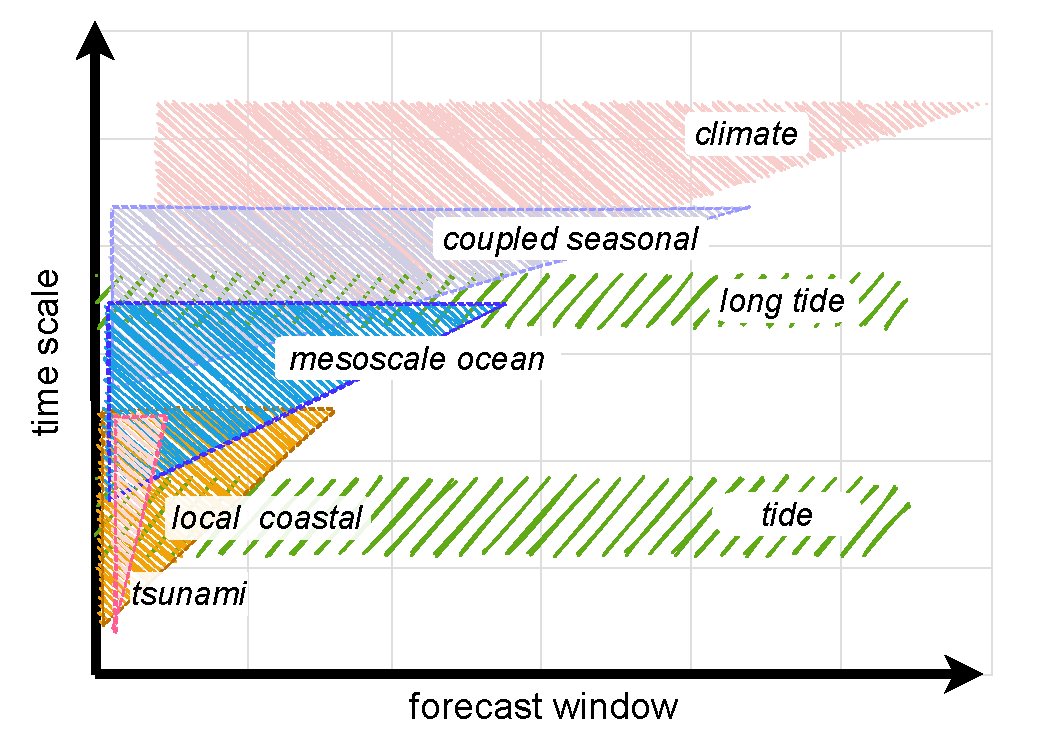
\includegraphics[height=0.8\textheight]{figures/diagrams/scales.pdf}
    %\end{figure} 
\end{frame}

%-----------------------------------------
\begin{frame}
\frametitle{Forecast systems and target scales}
    \begin{figure}      
     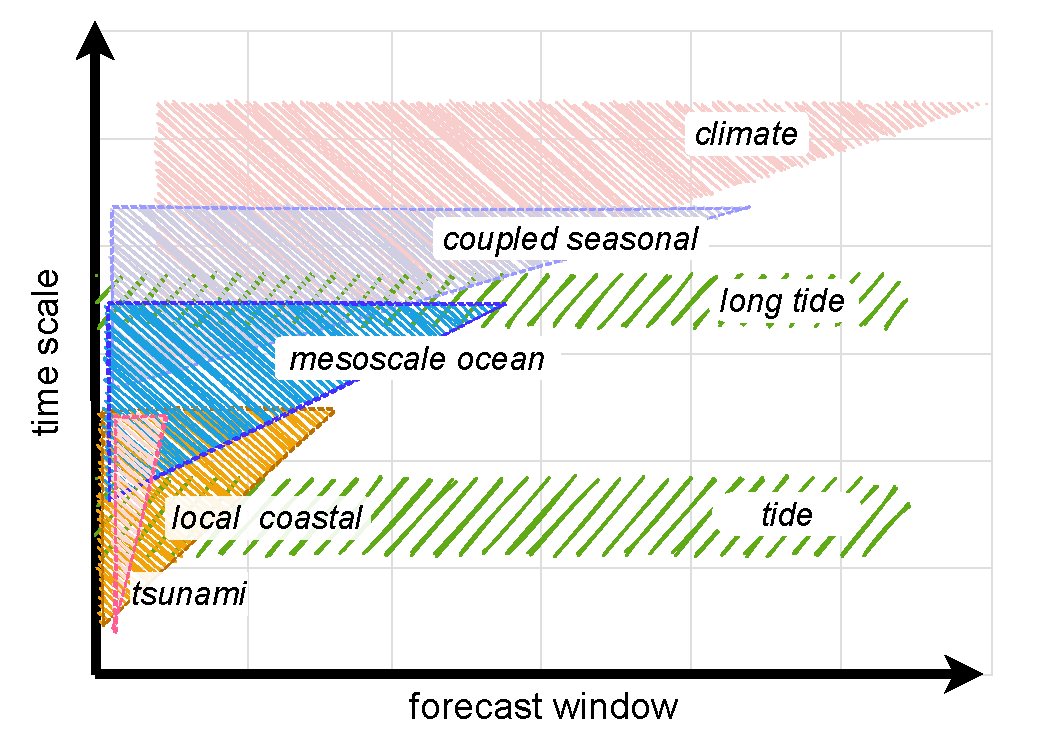
\includegraphics[height=0.8\textheight]{figures/diagrams/scales.pdf}
    \end{figure} 
\end{frame}

